% ****************************************************************************************
% ************************      ANALISIS VECTORIAL            ****************************
% ****************************************************************************************


% =======================================================
% =======         HEADER FOR DOCUMENT        ============
% =======================================================
    % *********   DOCUMENT ITSELF   **************
    \documentclass[12pt, fleqn]{report}                             %Type of docuemtn and size of font and left eq
    \usepackage[margin=1.2in]{geometry}                             %Margins and Geometry pacakge
    \usepackage{ifthen}                                             %Allow simple programming
    \usepackage{hyperref}                                           %Create MetaData for a PDF and LINKS!
    \usepackage{pdfpages}                                           %Create MetaData for a PDF and LINKS!
    \hypersetup{pageanchor=false}                                   %Solve 'double page 1' warnings in build
    \setlength{\parindent}{0pt}                                     %Eliminate ugly indentation
    \author{Oscar Andrés Rosas & Alan Enrique Ontiveros Salazar}    %Who I am

    % *********   LANGUAJE AND UFT-8   *********
    \usepackage[spanish]{babel}                                     %Please use spanish
    \usepackage[utf8]{inputenc}                                     %Please use spanish - UFT
    \usepackage[T1]{fontenc}                                        %Please use spanish
    \usepackage{textcmds}                                           %Allow us to use quoutes
    \usepackage{changepage}                                         %Allow us to use identate paragraphs
    \usepackage{anyfontsize}                                        %All the sizes

    % *********   MATH AND HIS STYLE  *********
    \usepackage{ntheorem, amsmath, amssymb, amsfonts}               %All fucking math, I want all!
    \usepackage{mathrsfs, mathtools, empheq}                        %All fucking math, I want all!
    \usepackage{centernot}                                          %Allow me to negate a symbol
    \decimalpoint                                                   %Use decimal point

    % *********   GRAPHICS AND IMAGES *********
    \usepackage{graphicx}                                           %Allow to create graphics
    \usepackage{wrapfig}                                            %Allow to create images
    \graphicspath{ {Graphics/} }                                    %Where are the images :D

    % *********   LISTS AND TABLES ***********
    \usepackage{listings, listingsutf8}                             %We will be using code here
    \usepackage[inline]{enumitem}                                   %We will need to enumarate
    \usepackage{tasks}                                              %Horizontal lists
    \usepackage{longtable}                                          %Lets make tables awesome
    \usepackage{booktabs}                                           %Lets make tables awesome
    \usepackage{tabularx}                                           %Lets make tables awesome
    \usepackage{multirow}                                           %Lets make tables awesome
    \usepackage{multicol}                                           %Create multicolumns

    % *********   HEADERS AND FOOTERS ********
    \usepackage{fancyhdr}                                           %Lets make awesome headers/footers
    \pagestyle{fancy}                                               %Lets make awesome headers/footers
    \setlength{\headheight}{16pt}                                   %Top line
    \setlength{\parskip}{0.5em}                                     %Top line
    \renewcommand{\footrulewidth}{0.5pt}                            %Bottom line

    \lhead{                                                         %Left Header
        \hyperlink{chapter.\arabic{chapter}}                        %Make a link to the current chapter
        {\normalsize{\textsc{\nouppercase{\leftmark}}}}             %And fot it put the name
    }

    \rhead{                                                         %Right Header
        \hyperlink{section.\arabic{chapter}.\arabic{section}}       %Make a link to the current chapter
            {\footnotesize{\textsc{\nouppercase{\rightmark}}}}      %And fot it put the name
    }

    \rfoot{\textsc{\small{\hyperref[sec:Index]{Ve al Índice}}}}     %This will always be a footer  

    \fancyfoot[L]{                                                  %Algoritm for a changing footer
        \ifthenelse{\isodd{\value{page}}}                           %IF ODD PAGE:
            {\href{https://compilandoconocimiento.com/yo/}          %DO THIS:
                {\footnotesize                                      %Send the page
                    {\textsc{Oscar Rosas y Alan Ontiveros}}}}       %Send the page
            {\href{https://compilandoconocimiento.com}              %ELSE DO THIS: 
                {\footnotesize                                      %Send the author
                    {\textsc{Compilando Conocimiento}}}}            %Send the author
    }
    
    
    
% ========================================
% ===========   COMMANDS    ==============
% ========================================

    % =====  GENERAL TEXT  ==========
    \newcommand \Quote {\qq}                                        %Use: \Quote to use quotes
    \newcommand \Over {\overline}                                   %Use: \Bar to use just for short
    \newcommand \ForceNewLine {$\Space$\\}                          %Use it in theorems for example
    
    \newenvironment{Indentation}[1][0.75em]                         %Use: \begin{Inde...}[Num]...\end{Inde...}
    {\begin{adjustwidth}{#1}{}}                                     %If you dont put nothing i will use 0.75 em
    {\end{adjustwidth}}                                             %This indentate a paragraph
    \newenvironment{SmallIndentation}[1][0.75em]                    %Use: The same that we upper one, just 
    {\begin{adjustwidth}{#1}{}\begin{footnotesize}}                 %footnotesize size of letter by default
    {\end{footnotesize}\end{adjustwidth}}                           %that's it


    % =====  GENERAL MATH  ==========
    \DeclareMathOperator \Space {\quad}                             %Use: \Space for a cool mega space
    \DeclareMathOperator \MiniSpace {\;}                            %Use: \Space for a cool mini space
    \newcommand \Such {\MiniSpace|\MiniSpace}                       %Use: \Such like in sets
    \newcommand \Also {\MiniSpace \text{y} \MiniSpace}              %Use: \Also so it's look cool
    \newcommand \Remember[1]{\Space\text{\scriptsize{#1}}}          %Use: \Remember so it's look cool

    \newtheorem{Theorem}{Teorema}[section]                          %Use: \begin{Theorem}[Name]\label{Nombre}...
    \newtheorem{Corollary}{Colorario}[Theorem]                      %Use: \begin{Corollary}[Name]\label{Nombre}...
    \newtheorem{Lemma}[Theorem]{Lemma}                              %Use: \begin{Lemma}[Name]\label{Nombre}...
    \newtheorem{Definition}{Definición}[section]                    %Use: \begin{Definition}[Name]\label{Nombre}...

    \newcommand{\Set}[1]{\left\{ \MiniSpace #1 \MiniSpace \right\}} %Use: \Set {Info}
    \newcommand{\Brackets}[1]{\left[ #1 \right]}                    %Use: \Brackets {Info} 
    \newcommand{\Wrap}[1]{\left( #1 \right)}                        %Use: \Wrap {Info} 
    \newcommand{\pfrac}[2]{\Wrap{\dfrac{#1}{#2}}}                   %Use: Put fractions in parentesis

    \newenvironment{MultiLineEquation}[1]                           %Use: To create MultiLine equations
        {\begin{equation}\begin{alignedat}{#1}}                     %Use: \begin{Multi..}{Num. de Columnas}
        {\end{alignedat}\end{equation}}                             %And.. that's it!
    \newenvironment{MultiLineEquation*}[1]                          %Use: To create MultiLine equations
        {\begin{equation*}\begin{alignedat}{#1}}                    %Use: \begin{Multi..}{Num. de Columnas}
        {\end{alignedat}\end{equation*}}                            %And.. that's it!


    % =====  LOGIC  ==================
    \DeclareMathOperator \doublearrow {\leftrightarrow}             %Use: \doublearrow for a double arrow
    \newcommand \lequal {\MiniSpace \Leftrightarrow \MiniSpace}     %Use: \lequal for a double arrow
    \newcommand \linfire {\MiniSpace \Rightarrow \MiniSpace}        %Use: \lequal for a double arrow
    \newcommand \longto {\longrightarrow}                           %Use: \longto for a long arrow

    % =====  NUMBER THEORY  ==========
    \DeclareMathOperator \Naturals  {\mathbb{N}}                     %Use: \Naturals por Notation
    \DeclareMathOperator \Primes    {\mathbb{P}}                     %Use: \Naturals por Notation
    \DeclareMathOperator \Integers  {\mathbb{Z}}                     %Use: \Integers por Notation
    \DeclareMathOperator \Racionals {\mathbb{Q}}                     %Use: \Racionals por Notation
    \DeclareMathOperator \Reals     {\mathbb{R}}                     %Use: \Reals por Notation
    \DeclareMathOperator \Complexs  {\mathbb{C}}                     %Use: \Complex por Notation

    % === LINEAL ALGEBRA & VECTORS ===
    \DeclareMathOperator \LinealTransformation {\mathcal{T}}        %Use: \LinealTransformation for a cool T
    \newcommand{\Mag}[1]{\left| #1 \right|}                         %Use: \Mag {Info} 

    \newcommand{\pVector}[1]{                                       %Use: \pVector {Matrix Notation} use parentesis
        \ensuremath{\begin{pmatrix}#1\end{pmatrix}}                 %Example: \pVector{a\\b\\c} or \pVector{a&b&c} 
    }
    \newcommand{\lVector}[1]{                                       %Use: \lVector {Matrix Notation} use a abs 
        \ensuremath{\begin{vmatrix}#1\end{vmatrix}}                 %Example: \lVector{a\\b\\c} or \lVector{a&b&c} 
    }
    \newcommand{\bVector}[1]{                                       %Use: \bVector {Matrix Notation} use a brackets 
        \ensuremath{\begin{bmatrix}#1\end{bmatrix}}                 %Example: \bVector{a\\b\\c} or \bVector{a&b&c} 
    }
    \newcommand{\Vector}[1]{                                        %Use: \Vector {Matrix Notation} no parentesis
        \ensuremath{\begin{matrix}#1\end{matrix}}                   %Example: \Vector{a\\b\\c} or \Vector{a&b&c}
    }
    \newcommand{\uVec}[1]{\boldsymbol{\hat{\textbf{$#1$}}}}         %Use: Unitary Vector


    % MATRIX
    \makeatletter                                                   %Example: \begin{matrix}[cc|c]
    \renewcommand*\env@matrix[1][*\c@MaxMatrixCols c] {             %WTF! IS THIS
        \hskip -\arraycolsep                                        %WTF! IS THIS
        \let\@ifnextchar\new@ifnextchar                             %WTF! IS THIS
        \array{#1}                                                  %WTF! IS THIS
    }                                                               %WTF! IS THIS
    \makeatother                                                    %WTF! IS THIS

    % TRIGONOMETRIC FUNCTIONS
    \newcommand{\Cos}[1]{\cos\Wrap{#1}}                             %Simple wrappers
    \newcommand{\Sin}[1]{\sin\Wrap{#1}}                             %Simple wrappers
    \newcommand{\Tan}[1]{tan\Wrap{#1}}                              %Simple wrappers
    
    \newcommand{\Sec}[1]{sec\Wrap{#1}}                              %Simple wrappers
    \newcommand{\Csc}[1]{csc\Wrap{#1}}                              %Simple wrappers
    \newcommand{\Cot}[1]{cot\Wrap{#1}}                              %Simple wrappers

    % === COMPLEX ANALYSIS ===
    \newcommand \Cis[1]  {\Cos{#1} + i \Sin{#1}}                    %Use: \Cis for cos(x) + i sin(x)
    \newcommand \pCis[1] {\Wrap{\Cis{#1}}}                          %Use: \pCis for the same ut parantesis
    \newcommand \bCis[1] {\Brackets{\Cis{#1}}}                      %Use: \bCis for the same to Brackets

    % ====== TRANSFORMS =====
    \newcommand{\FourierT}[1]{\mathscr{F} \left\{ #1 \right\} }     %Use: \FourierT {Funtion}
    \newcommand{\InvFourierT}[1]{\mathscr{F}^{-1}\left\{#1\right\}} %Use: \InvFourierT {Funtion}


    % === CALCULUS ===
    \newcommand \MiniDerivate[1][x] {\dfrac{d}{d #1}}               %Use: \MiniDerivate for simple use
    \newcommand \Derivate[2]                                        %Complete Derivate -- [f(x)][x]
        {\dfrac{d \; #1}{d #2}}                                     %Use: \Partial for simple use
    
    \newcommand \MiniUpperDerivate[2]                               %Mini Derivate High Orden Derivate -- [x][1]
        {\dfrac{d^{#2}}{d#1^{#2}}}                                  %Mini Derivate High Orden Derivate
    \newcommand \UpperDerivate[3]                                   %Complete High Orden Derivate -- [f(x)][x][1]
        {\dfrac{d^{#3} \; #1}{d#2^{#3}}}                            %Use: \UpperDerivate for simple use
    
    \newcommand \MiniPartial[1][x] {\dfrac{\partial}{\partial #1}} %Use: \MiniDerivate for simple use
    \newcommand \Partial[2]                                        %Complete Derivate -- [f(x)][x]
        {\dfrac{\partial \; #1}{\partial #2}}                      %Use: \Partial for simple use
    
    \newcommand \MiniUpperPartial[2]                                %Mini Derivate High Orden Derivate -- [x][1] 
        {\dfrac{\partial^{#2}}{\partial #1^{#2}}}                   %Mini Derivate High Orden Derivate
    \newcommand \UpperPartial[3]                                    %Complete High Orden Derivate -- [f(x)][x][1]
        {\dfrac{\partial^{#3} \; #1}{\partial#2^{#3}}}              %Use: \UpperDerivate for simple use

    \DeclareMathOperator \Evaluate  {\Big|}                         %Use: \Evaluate por Notation





    
    % =====  GENERAL COLOR  =========
    \definecolor{TealMD}{HTML}{009688}                              %Use: Color :D        
    \definecolor{IndigoMD}{HTML}{3F51B5}                            %Use: Color :D
    \definecolor{Green100MD}{HTML}{DCEDC8}                          %Use: Color :D
    \definecolor{Blue300MD}{HTML}{64B5F6}                           %Use: Color :D
    \definecolor{DeepPurpleMD}{HTML}{673AB7}                        %Use: Color :D
    \definecolor{BlueGrey100MD}{HTML}{CFD8DC}                       %Use: Color :D
    \definecolor{BlueGrey800MD}{HTML}{37474F}                       %Use: Color :D
    \definecolor{BlueGrey200MD}{HTML}{B0BEC5}                       %Use: Color :D
    \definecolor{Lime300MD}{HTML}{E6EE9C}                           %Use: Color :D

    \newenvironment{ColorText}[1]{                                  %Use: \begin{ColorText}
        \leavevmode\color{#1}\ignorespaces}                         %That's is!

    % =====  CODE EDITOR =========
    \lstdefinestyle{CompilandoStyle} {                              %This is Code Style
        backgroundcolor=\color{BlueGrey800MD},                      %Background Color  
        basicstyle=\tiny\color{white},                              %Font color
        commentstyle=\color{BlueGrey200MD},                         %Comment color
        stringstyle=\color{Lime300MD},                              %String color
        keywordstyle=\color{Blue300MD},                             %keywords color
        numberstyle=\tiny\color{TealMD},                            %Size of a number
        frame=shadowbox,                                            %Adds a frame around the code
        breakatwhitespace=true,                                     %Style   
        showstringspaces=false,                                     %Hate those spaces                  
        breaklines=true,                                            %Style                   
        keepspaces=true,                                            %Style                   
        numbers=left,                                               %Style                   
        numbersep=10pt,                                             %Style 
        xleftmargin=\parindent,                                     %Style 
        tabsize=4,                                                  %Style
        inputencoding=utf8/latin1                                   %Allow me to use special chars
    }
 
    \lstset{style=CompilandoStyle}                                  %Use this style




% =====================================================
% ============        COVER PAGE       ================
% =====================================================
\begin{document}
\begin{titlepage}
    
    % ============ TITLE PAGE STYLE  ================
    \definecolor{TitlePageColor}{cmyk}{1,.60,0,.40}                 %Simple colors
    \definecolor{ColorSubtext}{cmyk}{1,.50,0,.10}                   %Simple colors
    \newgeometry{left=0.25\textwidth}                               %Defines an Offset
    \pagecolor{TitlePageColor}                                      %Make it this Color to page
    \color{white}                                                   %General things should be white
    \newcommand{\Github}{https://github.com/compilandoconocimiento} %The general Parte

    % ===== MAKE SOME SPACE =========
    \vspace                                                         %Give some space
    \baselineskip                                                   %But we need this to up command

    % ============ NAME OF THE PROJECT  ============
    \makebox[0pt][l]{\rule{1.3\textwidth}{3pt}}                     %Make a cool line
    
    \href{\Github}                                                  %Link to project
    {\textbf{\textsc{\Huge Compilando Conocimiento}}}\\[2.7cm]      %Name of project   

    % ============ NAME OF THE BOOK  ===============
    \href{\Github/LibroAnalisisVectorial}                           %Link to Author
    {\fontsize{55}{66}\selectfont                                   %Set size
        \textbf{Análisis Vectorial}}\\[0.5cm]                       %Name of the book
    \textcolor{ColorSubtext}{\textsc{\Huge Cálculo}}                %Name of the general theme
    
    \vfill                                                          %Fill the space
    
    % ============ NAME OF THE AUTHOR  =============
    \href{https://github.com/alaneos777}                            %Link to Author
    {\LARGE \textsf{Alan Enrique Ontiveros Salazar}}                %Author

    % ===== MAKE SOME SPACE =========
    \vspace                                                         %Give some space
    \baselineskip                                                   %But we need this to up command
    
    {\large \textsf{Enero 2018}}                                    %Date

\end{titlepage}


% =====================================================
% ==========      RESTORE TO DOCUMENT      ============
% =====================================================
\restoregeometry                                                    %Restores the geometry
\nopagecolor                                                        %Use to restore the color to white






% =====================================================
% ========                INDICE              =========
% =====================================================
\tableofcontents{}
\label{sec:Index}

\clearpage




% //////////////////////////////////////////////////////////////////////////////////////////////////////////
% ///////////////////////////////////         SISTEMAS DE COORDENADAS      /////////////////////////////////
% //////////////////////////////////////////////////////////////////////////////////////////////////////////
\part{Sistemas de Coordenadass}
\clearpage


    % ===============================================================================
    % ===================           DEFINICIONES               ======================
    % ===============================================================================
    \chapter{Coordenadas Polares $(r, \theta)$}

        % ==============================================
        % ========         VECTORES BASE       =========
        % ==============================================
        \clearpage
        \section{Vectores Base}

            Sea $\vec r$ nuestro vector que va desde el origen del plano $X-Y$ hasta el Punto $A$,
            lo vamos a llamar un vector de posición:

            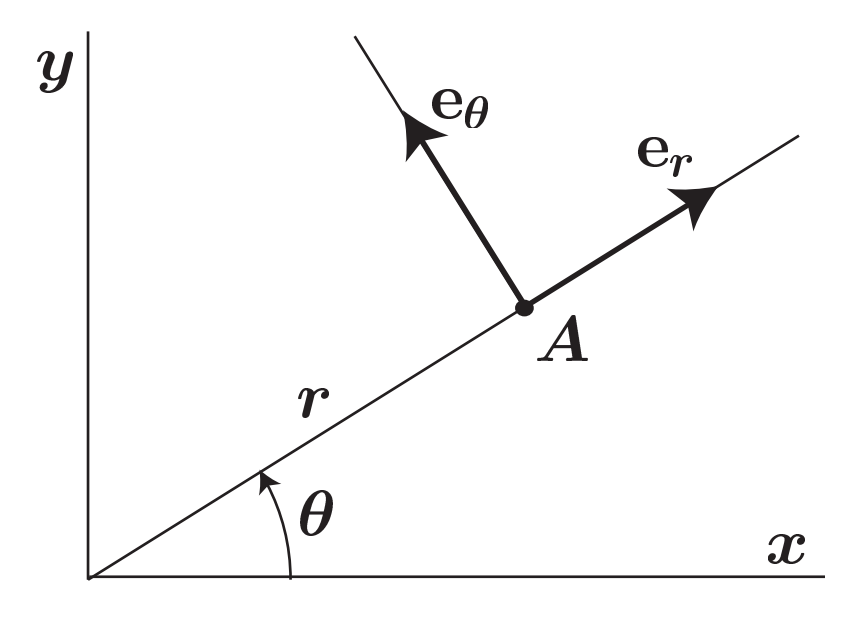
\includegraphics[width=0.50\textwidth]{CoordenadasPolares.png}

            Los vectores base, así como en coordenadas rectangulares ($\uVec{i}, \uVec{j}$) son dos
            vectores que denotaremos como: $\uVec{r}, \uVec{\theta}$. 

            Podemos entonces decir que el vector de posición tiene la magnitud igual a la distancia
            radial $r$ y tiene una dirección igual a $\uVec{r}$.
            Por lo tanto podemos decir que:
            \begin{equation}
                \vec{r} = r \cdot e_r
            \end{equation}






            % ========================================
            % =========     COSAS - IDEAS      =======
            % ========================================
            \subsection{Ideas sobre esos Vectores Base}

                Estos vectores base son bastante diferente a lo que tu verías en los vectores
                base de la base rectangulas, nuestros queridos amigos ($\uVec{i}, \uVec{j}$)
                pues sin importar de que vector estemos hablando, los vectores base con siempre 
                los mismo.
                \textbf{Esto no pasa en la Base Polar}.



            % ========================================
            % ====      CAMBIO A LAS CANONICAS      ==
            % ========================================
            \clearpage
            \subsection{Cambio de Base con Canónicas}
                Tenemos una propiedad muy importante que nos dice que:
                \begin{itemize}
                    \item $\uVec{r}      =  \Cos{\theta}\uVec{i} + \Sin{\theta} \uVec{j}$
                    \item $\uVec{\theta} = -\Sin{\theta}\uVec{i} + \Cos{\theta} \uVec{j}$
                \end{itemize}


                Y también que:
                \begin{itemize}
                    \item $\uVec{i} = \Cos{\theta}\uVec{r} - \Sin{\theta} \uVec{\theta}$
                    \item $\uVec{j} = \Sin{\theta}\uVec{r} + \Cos{\theta} \uVec{\theta}$
                \end{itemize}


            % ========================================
            % ====      MATRIZ DE CAMBIO DE BASE    ==
            % ========================================
            \subsection{Matriz de Cambio de Base con Canónicas}
                Tenemos una propiedad muy importante que nos dice que:
                \begin{equation}
                    \pVector{r \\ \theta} = 
                        \pVector{
                            \Cos{\theta} &+& \Sin{\theta} \\
                           -\Sin{\theta} &+& \Cos{\theta} 
                        }
                        \pVector{x \\ y}
                \end{equation}

                Y también que:
                \begin{equation}
                    \pVector{x \\ y} = 
                        \pVector{
                            \Cos{\theta} &+& -\Sin{\theta} \\
                            \Sin{\theta} &+& \Cos{\theta} 
                        }
                        \pVector{r \\ \theta}
                \end{equation}             


            % ========================================
            % ====  DERIVACION VECTORES UNITARIOS   ==
            % ========================================
            \clearpage
            \subsection{Derivación de Vectores Unitarios}

                \begin{itemize}
                    
                    \item 
                        $\Derivate{\uVec{r}}{r} = \vec{0}$
                        
                        % ======== DEMOSTRACION ========
                        \begin{SmallIndentation}[1em]
                            \textbf{Ideas}:

                            Ahora nota que no importa cuanto cambia $r$ en el vector $(r, \theta)$, el vector
                            unitario $\uVec{r}$ no cambia por mas que $r$ cambie, por lo tanto es el cero
                            vector.

                            Esto también se comprueba pues:
                            \begin{equation*}
                                \Derivate{\uVec{r}}{r}                                        =
                                \Derivate{\Cos{\theta}\uVec{i} + \Sin{\theta} \uVec{j}}{r}   =
                                \vec{0}
                            \end{equation*}
                        \end{SmallIndentation}

                    \item
                        $\Derivate{\uVec{\theta}}{r} = \vec{0}$
                        
                        % ======== DEMOSTRACION ========
                        \begin{SmallIndentation}[1em]
                            \textbf{Ideas}:

                            Ahora nota que no importa cuanto cambia $r$ en el vector $(r, \theta)$, el vector
                            unitario $\uVec{\theta}$ no cambia por mas que $r$ cambie, por lo tanto es el
                            cero vector.

                            Esto también se comprueba pues:
                            \begin{equation*}
                                \Derivate{\uVec{r}}{r}                                        =
                                \Derivate{-\Sin{\theta}\uVec{i} + \Cos{\theta} \uVec{j}}{r}  =
                                \vec{0}
                            \end{equation*}

                        \end{SmallIndentation}


                    \item
                        $\Derivate{\uVec{r}}{\theta} = \uVec{\theta}$
                        
                        % ======== DEMOSTRACION ========
                        \begin{SmallIndentation}[1em]
                            \textbf{Ideas}:

                            Esta idea es bastante fácil de demostrar usando la base rectangular:

                            \begin{MultiLineEquation*}{2}
                                \Derivate{\uVec{r}}{\theta} 
                                        &= \Derivate{\Cos{\theta}\uVec{i} + \Sin{\theta} \uVec{j}}{\theta}   \\
                                        &=  \Derivate{\Cos{\theta}}{\theta}\uVec{i}
                                                +
                                            \Derivate{\Sin{\theta}}{\theta}\uVec{j}                            \\
                                        &= -\Sin{\theta}\uVec{i} + \Cos{\theta} \uVec{j}
                                        &= \uVec{\theta}
                            \end{MultiLineEquation*}
                            
                        \end{SmallIndentation}

                    \item
                        $\Derivate{\uVec{\theta}}{\theta} = -\uVec{r}$
                        
                        % ======== DEMOSTRACION ========
                        \begin{SmallIndentation}[1em]
                            \textbf{Ideas}:

                            Esta idea es bastante fácil de demostrar usando la base rectangular:

                            \begin{MultiLineEquation*}{2}
                                \Derivate{\uVec{r}}{\theta} 
                                        &= \Derivate{-\Sin{\theta}\uVec{i} + \Cos{\theta} \uVec{j}}{\theta}  \\
                                        &=  \Derivate{-\Sin{\theta}}{\theta}\uVec{i}
                                                +
                                            \Derivate{\Cos{\theta}}{\theta}\uVec{j}                            \\
                                        &= -\Cos{\theta}\uVec{i} + -\Sin{\theta} \uVec{j}                     
                                        &= -\uVec{r}
                            \end{MultiLineEquation*}
                            
                        \end{SmallIndentation}
                        



                \end{itemize}



            % ============================================
            % ====  DERIVACION DE R CON RESPECTO A T =====
            % ============================================
            \clearpage
            \subsection{Derivación con respecto al tiempo $\Derivate{\uVec{r}}{t}$}

                Supongase que tenemos un vector de posición $\vec{r}$ que se mueve libremente con respecto
                al tiempo en todas las direcciones posibles, entonces tenemos que:
                
                % ======== DEMOSTRACION ========
                \begin{SmallIndentation}[1em]
                    \textbf{Ideas}:

                    Sea $\vec{r} = r \uVec{r}$ entonces podemos decir que:
                    \begin{MultiLineEquation}{2}
                        \Derivate{\vec{r}}{t}   &= \MiniDerivate{t} r \uVec{r}                                  \\
                                                &= r \Derivate{\uVec{r}}{t} + \Derivate{r}{t}\uVec{r}                   
                    \end{MultiLineEquation}

                    Y ahora recuerda que:

                    \begin{MultiLineEquation*}{3}
                        \Derivate{\uVec{r}}{t}
                                &= \MiniDerivate{t} \Wrap{\Cos{\theta} \uVec{i} + \Sin{\theta} \uVec{j}}        &&
                                \Remember{La forma de colocar a $\uVec{r}$ en coord. rectangulares}             \\
                                &= \Wrap{-\Sin{\theta} \uVec{i} + \Cos{\theta} \uVec{j}} \Derivate{\theta}{t}   &&
                                \Remember{Derivamos como siempre}                                               \\
                                &= \uVec{\theta} \Derivate{\theta}{t}                                           &&
                                \Remember{Recuerda que ya demostramos esto}                                     \\
                    \end{MultiLineEquation*}

                    Por lo tanto tenemos que:
                    \begin{MultiLineEquation}{2}
                        \Derivate{\vec{r}}{t}   &= \MiniDerivate{t} r \uVec{r}                                              \\
                                                &= r \Derivate{\uVec{r}}{t} + \Derivate{r}{t}\uVec{r}                       \\
                                                &= r \uVec{\theta} \Derivate{\theta}{t} + \Derivate{r}{t}\uVec{r}           \\
                                                &= \Wrap{r \Derivate{\theta}{t}} \uVec{\theta} + \Derivate{r}{t} \uVec{r}                  
                    \end{MultiLineEquation}

                    
                \end{SmallIndentation}































            

\end{document}
